%Este trabalho está licenciado sob a Licença Atribuição-CompartilhaIgual 4.0 Internacional Creative Commons. Para visualizar uma cópia desta licença, visite http://creativecommons.org/licenses/by-sa/4.0/deed.pt_BR ou mande uma carta para Creative Commons, PO Box 1866, Mountain View, CA 94042, USA.

\chapter{Sistema de coordenadas}\label{cap_scoord}
\thispagestyle{fancy}

A geometria analítica é uma área interdisciplinar da matermática que faz o estudo de objetos da geometria através de estruturas algébricas (equações e inequações algébricas). Para tanto, o primeiro passo é a construção (definição) de um sistema de coordenadas, no qual os objetos geométricos serão referenciados.

\section{Sistema de coordenadas no espaço}\label{cap_scoord_sec_scoord}

Um sistema de coordenadas no espaço (euclidiano) é constituído de um ponto $O$ e uma base de vetores $B = (\vec{e}_1, \vec{e}_2, \vec{e}_3)$ no espaço. Dado um tal sistema, temos que cada ponto $P$ determina de forma única um vetor $\overrightarrow{OP} = (x,y,z)$ e vice-versa. Assim sendo, definimos que o ponto $P$ tem coordenadas $(x,y,z)$. Veja a figura abaixo.

\begin{figure}[H]
  \centering
  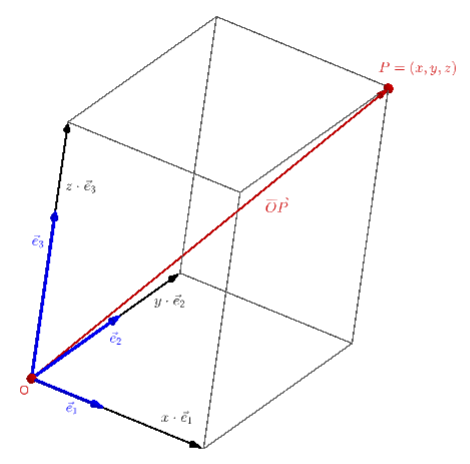
\includegraphics[width=0.8\textwidth]{cap_scoord/dados/fig_scoord/fig}
  \caption{Ilustração de um sistema de coordenadas no espaço.}
  \label{fig:scoord}
\end{figure}

O ponto $O$ é chamado de \emph{origem} (do sistema de coordenadas) e tem coordenadas $O=(0,0,0)$. Dado um ponto $P=(x,y,z)$, chama-se $x$ de sua \emph{abscissa}, $y$ de sua \emph{ordenada} e $z$ de sua \emph{cota}. As retas que passam por $O$ e têm, respectivamente, as mesmas direções de $\vec{e}_1$, $\vec{e}_2$ e $\vec{e}_3$ são chamadas de \emph{eixo das abscissas}, \emph{eixo das ordenadas} e \emph{eixo das cotas}. Os planos que contém $O$ e representantes de dois vetores da base $B$ são chamados de \emph{planos coordenados}.

\begin{figure}[H]
  \centering
  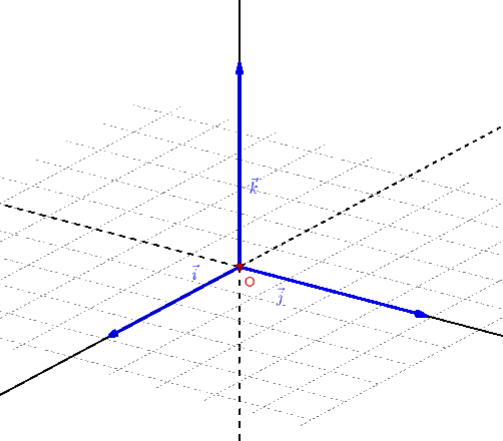
\includegraphics[width=0.7\textwidth]{./cap_scoord/dados/fig_sis_coord_orto/fig}
  \caption{Ilustração de um sistema de coordenadas ortonormal.}
  \label{fig:sis_coord_orto}
\end{figure}

Salvo explicitado ao contrário, trabalharemos com um \emph{sistema de coordenadas ortonormal}, i.e. sistema cuja base $B = (\vec{i},\vec{j},\vec{k})$ seja ortonormal. Mais ainda, estaremos assumindo que a base é positiva. Veja a Figura \ref{fig:sis_coord_orto}.

\begin{obs}\normalfont{(Relação entre pontos e vetores)}
  Seja dado um vetor $\overrightarrow{AB}$. Sabendo as coordenadas dos pontos $A = (x_A,y_A,z_A)$ e $B = (x_B,y_B,z_B)$, temos que as coordenadas do vetor $\overrightarrow{AB}$ são:
  \begin{align}
    \overrightarrow{AB} &= \overrightarrow{AO} + \overrightarrow{OB}\\
                        &= -\overrightarrow{OA} + \overrightarrow{OB}\\
                        &= -(x_A,y_A,z_A)+(x_B,y_B,z_B)\\
                        &= (x_B-x_A,y_B-y_A,z_B-z_A).
  \end{align}
  Em uma linguagem menos formal, podemos dizer que as coordenadas de $\overrightarrow{AB}$ é a resultante das coordenadas do ponto final menos as coordenadas do ponto de partida. Veja a figura abaixo.

\begin{figure}[H]
  \centering
  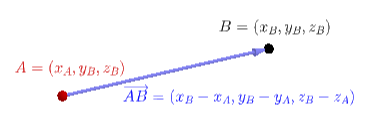
\includegraphics[width=0.6\textwidth]{./cap_scoord/dados/fig_scoord_vec_pt/fig}
  \caption{Relação entre as coordenadas dos pontos de partida e de chegada de um vetor.}
  \label{fig:scoord_vec_pt}
\end{figure}  
\end{obs}

\begin{ex}
  Dados os pontos $A = (-1,1,2)$ e $B = (3,-1,0)$, temos que o vetor $\overrightarrow{AB}$ tem coordenadas:
  \begin{equation}
    \overrightarrow{AB} = (3-(-1),-1-1,0-2) = (4,-2,-2).
  \end{equation}
\end{ex}

\begin{obs}\normalfont{(Ponto médio de um segmento)}
  Dados os pontos $A = (x_A,y_A,z_A)$ e $B = (x_B,y_B,z_B)$, podemos calcular as coordenadas do ponto médio $M = (x_M,y_M,z_M)$ do segmento $AB$. Veja a figura abaixo.

\begin{figure}[H]
  \centering
  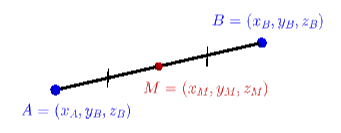
\includegraphics[width=0.6\textwidth]{./cap_scoord/dados/fig_scoord_pm/fig}
  \caption{Coordenadas do ponto médio de um segmento.}
  \label{fig:scoord_pm}
\end{figure}  

  Do fato de que $\overrightarrow{AM} = \overrightarrow{MB}$, temos
  \begin{equation}
    (x_M-x_A,y_M-y_A,z_M-z_A)=(x_B-x_M,y_B-y_M,z_B-z_M),
  \end{equation}
  Logo, segue que
  \begin{align}
    x_M-x_A &= x_B-x_M\\
    y_M-y_A &= y_B-y_M\\
    z_M-z_A &= z_B-z_M
  \end{align}
  ou, equivalentemente,
  \begin{align}
    2x_M &= x_A+x_B\\
    2y_M &= y_A+y_B\\
    2z_M &= z_A+z_B
  \end{align}
  Portanto, concluímos que
  \begin{align}
    x_M &= \frac{x_A+x_B}{2}\\
    y_M &= \frac{y_A+y_B}{2}\\
    z_M &= \frac{z_A+z_B}{2}
  \end{align}  
  Logo, temos
  \begin{equation}
  M = \left(\frac{x_A+x_B}{2},\frac{y_A+y_B}{2},\frac{z_A+z_B}{2}\right)
\end{equation}
\end{obs}

\begin{ex}
  Dados os pontos $A = (-1,1,2)$ e $B = (3,-1,0)$, temos que o ponto médio do segmento $AB$ tem coordenadas:
  \begin{align}
    M &= \left(\frac{-1+3}{2},\frac{1+(-1)}{2},\frac{2+0}{2}\right)\\
    &= (1,0,1).
  \end{align}
\end{ex}

\subsection*{Exercícios resolvidos}

\begin{exeresol}
  Sejam $A = (-1,2,1)$, $B = (1,-2,0)$ e $C = (x,2,2)$ vértices consecutivos de um triângulo isósceles, cujos lados $AC$ e $BC$ são congruentes. Determine o valor de $x$.
\end{exeresol}
\begin{resol}
  Sendo os lados $AC$ e $BC$ congruentes, temos $|\overrightarrow{AC}| = |\overrightarrow{BC}|$. As coordenadas de $\overrightarrow{AC}$ são
  \begin{equation}
    \overrightarrow{AC} = (x-(-1),2-2,2-1) = (x+1,0,1)
  \end{equation}
  e as coordenadas de $\overrightarrow{BC}$ são
  \begin{equation}
    \overrightarrow{BC} = (x-1,2-(-2),2-0) = (x-1,4,2).
  \end{equation}
  Então, temos
  \begin{align}
    |\overrightarrow{AC}| = |\overrightarrow{BC}| &\Rightarrow \sqrt{(x+1)^2+0^2+1^2} = \sqrt{(x-1)^2+4^2+2^2}\\
                                                  &\Rightarrow (x+1)^2+0^2+1^2 = (x-1)^2+4^2+2^2\\
                                                  &\Rightarrow x^2+2x+1+1 = x^2-2x+1+16+4\\
                                                  &\Rightarrow 4x = 19\\
                                                  &\Rightarrow x = \frac{19}{4}.
  \end{align}
\end{resol}

\begin{exeresol}
  Sejam $A = (-1,2,1)$, $B = (1,-2,0)$  e $M$ o ponto médio do intervalo $AB$. Determine as coordenadas do ponto $P$ de forma que $2AP = AM$.
\end{exeresol}
\begin{resol}
  As coordenadas do ponto médio são
  \begin{equation}
    M = \left(\frac{-1+1}{2},\frac{2+(-2)}{2},\frac{1+0}{2}\right) = \left(0,0,\frac{1}{2}\right).
  \end{equation}
  Agora, denotando $P = (x_P,y_P,z_P)$, temos
  \begin{align}
    2AP = AM &\Rightarrow 2(x_P-(-1),y_P-2,z_P-1) = \left(0-(-1),0-2,\frac{1}{2}-1\right)\\
             &\Rightarrow (2x_p+2,2y_P-4,2z_P-2) = \left(1,-2,-\frac{1}{2}\right).
  \end{align}
  Portanto
  \begin{align}
    & 2x_P+2 = 1 \Rightarrow x_P = -\frac{1}{2}\\
    & 2y_P-4 = -2 \Rightarrow y_P = 1\\
    & 2z_P-2 = -\frac{1}{2} \Rightarrow z_P = \frac{3}{4}.
  \end{align}
  Logo, $P = (-1/2,1,3/4)$.
\end{resol}

\subsection*{Exercícios}

\emconstrucao

\section{Equações da reta}\label{cap_ert_sec_eqsreta}

\subsection{Equação vetorial de uma reta}

Seja $r$ uma reta dada, $\vec{v}$ um vetor paralelo a $r$ e $A$ um ponto de $r$ (veja a Figura~\ref{fig:er_vet}). Assim sendo, $P$ é um ponto de $r$ se, e somente se, existe $\lambda\in\mathbb{R}$ tal que
\begin{equation}
  \overrightarrow{AP} = \lambda\vec{v}.
\end{equation}
Esta é chamada \emph{equação vetorial da reta} $r$.

\begin{figure}[H]
  \centering
  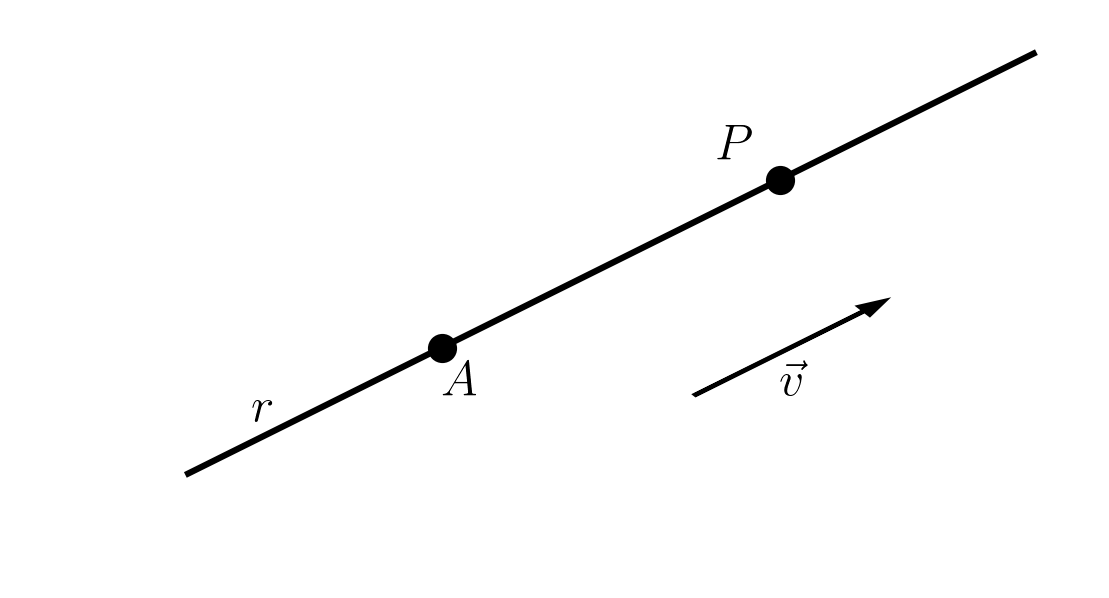
\includegraphics[width=0.5\textwidth]{./cap_er/dados/fig_er_vet/fig_er_vet}
  \caption{Equação vetorial de uma reta.}
  \label{fig:er_vet}
\end{figure}

Observe que para obtermos uma equação vetorial de uma dada reta, podemos escolher qualquer ponto $A\in r$ e qualquer vetor $\vec{v}\parallel r$, $\vec{v}\neq\vec{0}$. O vetor $\vec{v}$ escolhido é chamado de \emph{vetor diretor}.

\begin{ex}\label{ex:er_vet}
  Seja $r$ a reta que passa pelos pontos $A=(-1,-1,-2)$ e $B = (2,1,3)$ (veja a Figura \ref{fig:ex_er_vet}). O vetor
  \begin{equation}
    \vec{v} = \overrightarrow{AB} = (2-(-1),1-(-1),3-(-2)) = (3,2,5)
  \end{equation}
  é um vetor diretor de $r$. Desta forma, uma equação vetorial da reta $r$ é
  \begin{equation}
    \overrightarrow{AP} = \lambda\vec{v}.
  \end{equation}
  \begin{figure}[H]
    \centering
    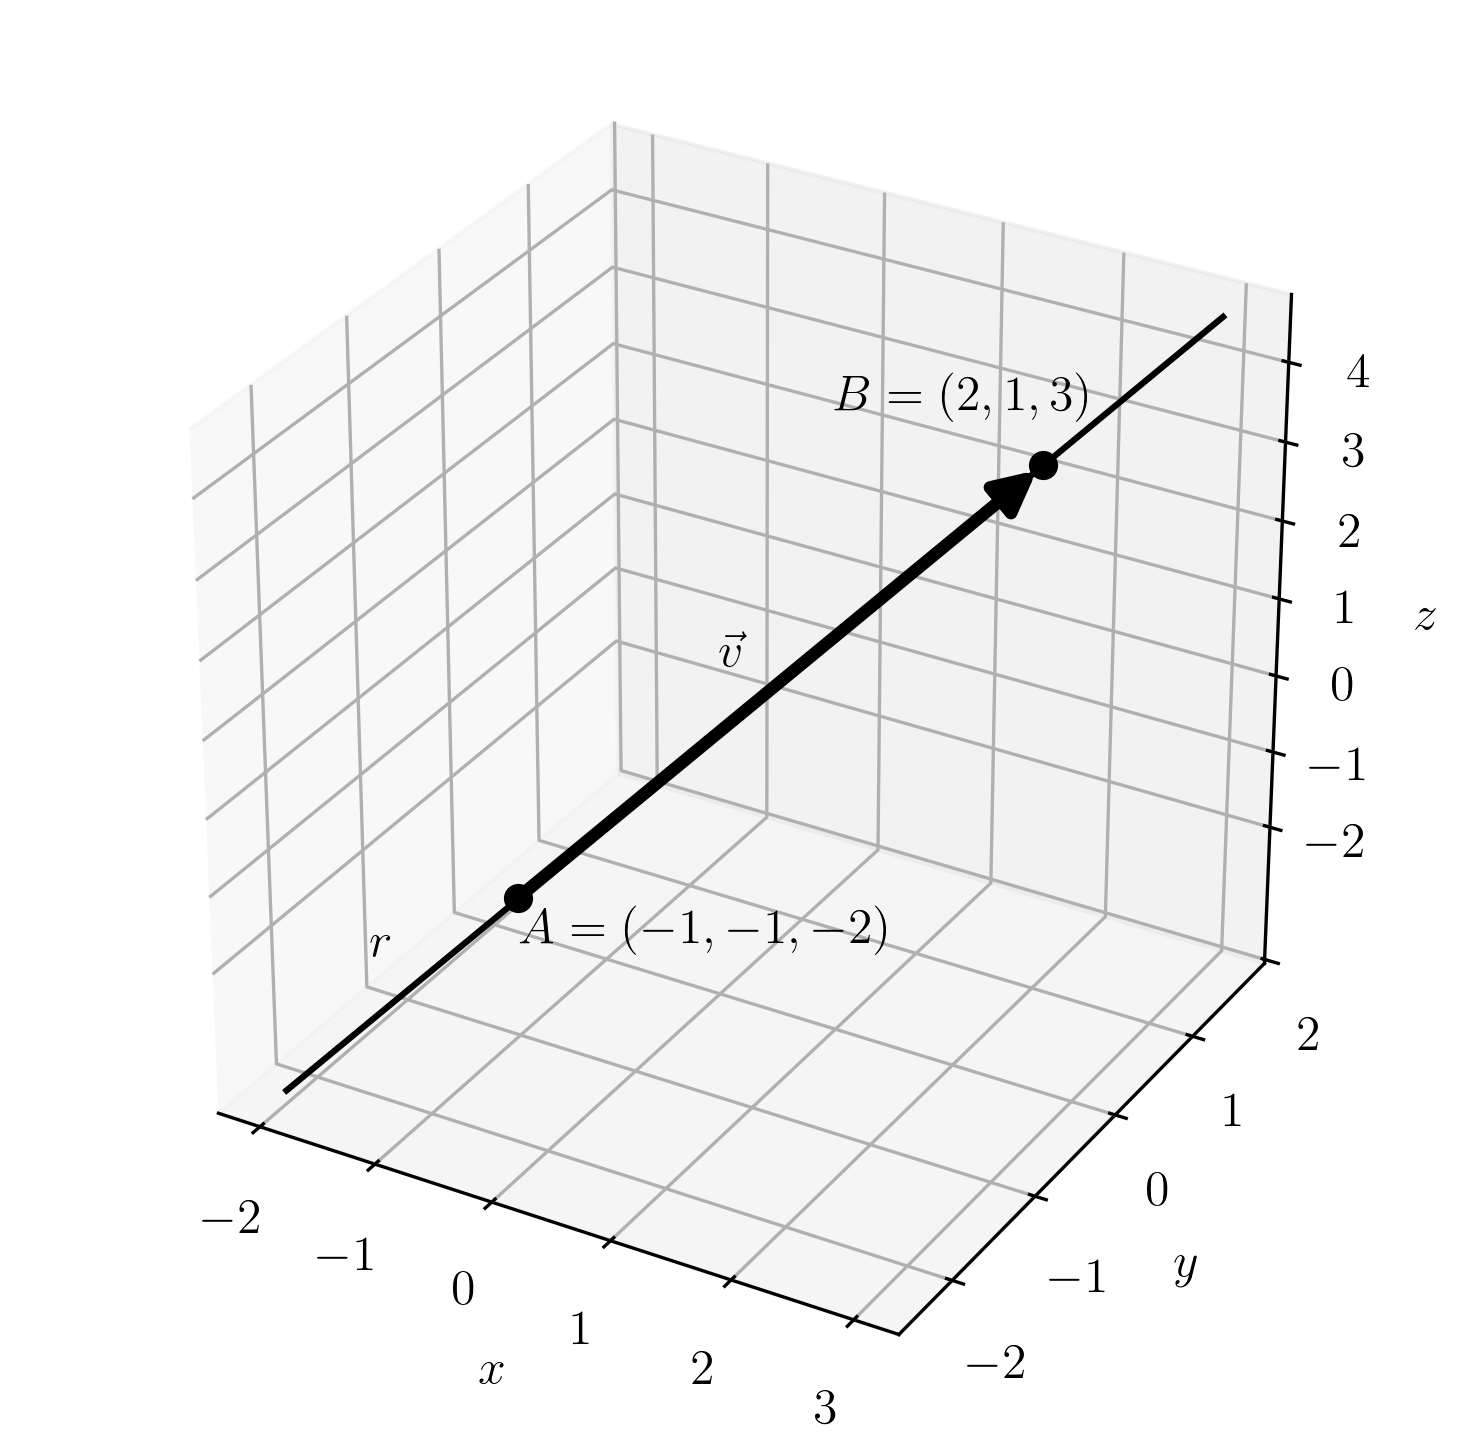
\includegraphics[width=0.7\textwidth]{./cap_er/dados/fig_ex_er_vet/fig_ex_er_vet}
    \caption{Esboço da reta discutida no Exemplo \ref{ex:er_vet}.}
    \label{fig:ex_er_vet}
  \end{figure}  
\end{ex}

\subsection{Equações paramétricas de uma reta}

Seja $r$ uma reta que passa pelo ponto $A = (x_A,y_A,z_A)$ e tenha vetor diretor $\vec{v} = (v_1,v_2,v_3)$. Assim, $P = (x,y,z)\in r$ se, e somente se, existe $\lambda\in\mathbb{R}$ tal que
\begin{equation}
  \overrightarrow{AP} = \lambda\vec{v}.
\end{equation}
Equivalentemente,
\begin{equation}
  (x-x_A,y-y_A,z-z_A) = \lambda (v_1,v_2,v_3).
\end{equation}
Então,
\begin{align}
  x-x_A &= \lambda v_1,\\
  y-y_A &= \lambda v_2,\\
  z-z_A &= \lambda v_3,
\end{align}
donde
\begin{align}
  x &= x_A + \lambda v_1,\\
  y &= y_A + \lambda v_2,\\
  z &= z_A + \lambda v_3,
\end{align}
as quais são chamadas de \emph{equações paramétricas} da reta $r$.

\begin{ex}\label{ex:ex_er_par}
  A reta $r$ discutida no Exemplo \ref{ex:er_vet} tem equações paramétricas
  \begin{align}
    x &= -1 + 3\lambda,\\
    y &= -1 + 2\lambda,\\
    z &= -2 + 5\lambda.
  \end{align}
  De fato, tomando $\lambda = 0$, temos $(x,y,z) = (-1,-1,-2) = A\in r$. E, tomado $\lambda = 1$, temos $(x,y,z) = (-1+3,-1+2,-2+5) = (2,1,3) = B\in r$. Ou seja, as equações paramétricas acima representam a reta que passa pelos pontos $A$ e $B$.

  \ifispython
  Com o \verb+Sympy+, podemos plotar o gráfico de $r$ usando o seguinte código\footnote{Veja a Observação \ref{obs:cap_er_py}.}:
\begin{verbatim}
var('lbda',real=True)
plot3d_parametric_line(-1+3*lbda,-1+2*lbda,-2+5*lbda,(lbda,-1,2))
\end{verbatim}
  \fi
\end{ex}

\subsection{Equações da reta na forma simétrica}

Seja $r$ uma reta que passa pelo ponto $A = (x_A,y_A,z_A)$ e tem $\vec{v} = (v_1,v_2,v_3)$ como vetor diretor. Então, $r$ tem as equações paramétricas
\begin{align}
  x &= x_A + v_1\lambda,\\
  y &= y_A + v_2\lambda,\\
  z &= z_A + v_3\lambda.
\end{align}
Isolando $\lambda$ em cada uma das equações, obtemos
\begin{equation}
  \frac{x-x_A}{v_1} = \frac{y-y_A}{v_2} = \frac{z-z_A}{v_3},
\end{equation}
as quais são as \emph{equações da reta na forma simétrica}.

\begin{ex}
  No Exemplo \ref{ex:ex_er_par}, consideramos a reta $r$ de equações paramétricas
  \begin{align}
    x &= -1 + 3\lambda,\\
    y &= -1 + 2\lambda,\\
    z &= -2 + 5\lambda.    
  \end{align}
  Para obtermos as equações de $r$ na forma simétrica, basta isolarmos $\lambda$ em cada equação. Com isso, obtemos
  \begin{equation}
    \frac{x+1}{3} = \frac{y+1}{2} = \frac{z+2}{5}.
  \end{equation}
\end{ex}

\subsection{Exercícios resolvidos}

\begin{exeresol}
  Seja $r$ a reta que passa pelo ponto $A = (-1,-1,-2)$ e tem $\vec{v} = (3,2,5)$ como vetor diretor. Determine o valor de $x$ de forma que $P = (x,0,1/2)$ seja um ponto de $r$.
\end{exeresol}
\begin{resol}
  $P = (x,0,1/2)$ é um ponto de $r$ se, e somente se, existe $\lambda\in\mathbb{R}$ tal que
  \begin{equation}
    \overrightarrow{AP} = \lambda\vec{v}.
  \end{equation}
  Ou seja,
  \begin{equation}
    \left(x-(-1),0-(-1),\frac{1}{2}-(-2)\right) = \lambda (3,2,5).
  \end{equation}
  Ou, equivalentemente,
  \begin{equation}
    \left(x+1,1,\frac{5}{2}\right) = \lambda (3,2,5).
  \end{equation}
  Usando a segunda coordenada destes vetores, temos
  \begin{equation}
    1 = \lambda\cdot 2 \Rightarrow \lambda = \frac{1}{2}.
  \end{equation}
  Assim, da primeira coordenada dos vetores, temos
  \begin{align}
    x+1 = \lambda 3 &\Rightarrow x+1 = \frac{3}{2}\\
                    &\Rightarrow x = \frac{3}{2}-1 = \frac{1}{2}.
  \end{align}
\end{resol}

\begin{exeresol}
  Seja $r$ a reta de equações paramétricas
  \begin{align}
    x &= 1 -\lambda,\\
    y &= \lambda,\\
    z &= -3.
  \end{align}
  Determine uma equação vetorial de $r$.
\end{exeresol}
\begin{resol}
  Nas equações paramétricas de uma reta, temos que os coeficientes constantes estão associados a um ponto da reta. Os coeficientes de $\lambda$ estão associados a um vetor diretor. Assim sendo, das equações paramétricas da reta $r$, temos que $A = (1,0,-3)\in r$ e $\vec{v} = (-1,1,0)$ é um vetor diretor. Logo, temos que a reta $r$ tem equação vetorial
  \begin{equation}
    \overrightarrow{AP} = \lambda\vec{v},
  \end{equation}
  com $A = (1,0,3)$ e $\vec{v} = (-1,1,0)$.
\end{resol}

\begin{exeresol}
  Sabendo que $r$ é uma reta que passa pelos pontos $A = (2,-3,1)$ e $B = (-1,1,0)$, determine o valor de $t$ tal que
  \begin{align}
    x = 2 + t\lambda,\\
    y = -2 + 4\lambda,\\
    z = 1 -\lambda,
  \end{align}
  sejam equação paramétricas de $r$.
\end{exeresol}
\begin{resol}
  Para que estas sejam equações paramétricas de $r$, é necessário que $\vec{v} = (t,4,-1)$ seja um vetor diretor de $r$. Em particular, $\vec{v} \parallel \overrightarrow{AB}$. Logo, existe $\beta\in\mathbb{R}$ tal que
  \begin{equation}
    (t,4,-1) = \beta (-1-2,1-(-3),0-1) = \beta (-3,4,-1).
  \end{equation}
  Das segunda e terceira coordenadas, temos $\beta = 1$. Daí, comparando pela primeira coordenada, temos
  \begin{equation}
    t = -3\beta \Rightarrow t = -3.
  \end{equation}
\end{resol}

\begin{exeresol}\label{exeresol:er_sim}
  Seja $r$ uma reta, cujas equações na forma simétrica são
  \begin{equation}
    \frac{x+1}{2} = \frac{y-2}{3} = \frac{1-z}{2}.
  \end{equation}
  Determine equações paramétricas desta reta e faça um esboço de seu gráfico.
\end{exeresol}
\begin{resol}
  Podemos obter equações paramétricas desta reta a partir de suas equações na forma simétrica. Para tanto, basta tomar o parâmetro $\lambda$ tal que
  \begin{align}
    \lambda &= \frac{x+1}{2},\\
    \lambda &= \frac{y-2}{3},\\
    \lambda &= \frac{1-z}{2}.
  \end{align}
  Daí, isolando $x$, $y$ e $z$ em cada uma destas equações, obtemos
  \begin{align}
    x &= -1 + 2\lambda,\\
    y &= 2 + 3\lambda,\\
    z &= 1 - 2\lambda.
  \end{align}
  Para fazermos um esboço do gráfico desta reta, basta traçarmos a reta que passa por dois de seus pontos. Por exemplo, tomando $\lambda = 0$, temos $A = (-1,2,1)\in r$. Agora, tomando $\lambda = 1$, temos $B = (1,5,-1)\in r$. Desta forma, obtemos o esboço dado na Figura \ref{fig:exeresol_er_sim}.

  \begin{figure}[H]
    \centering
    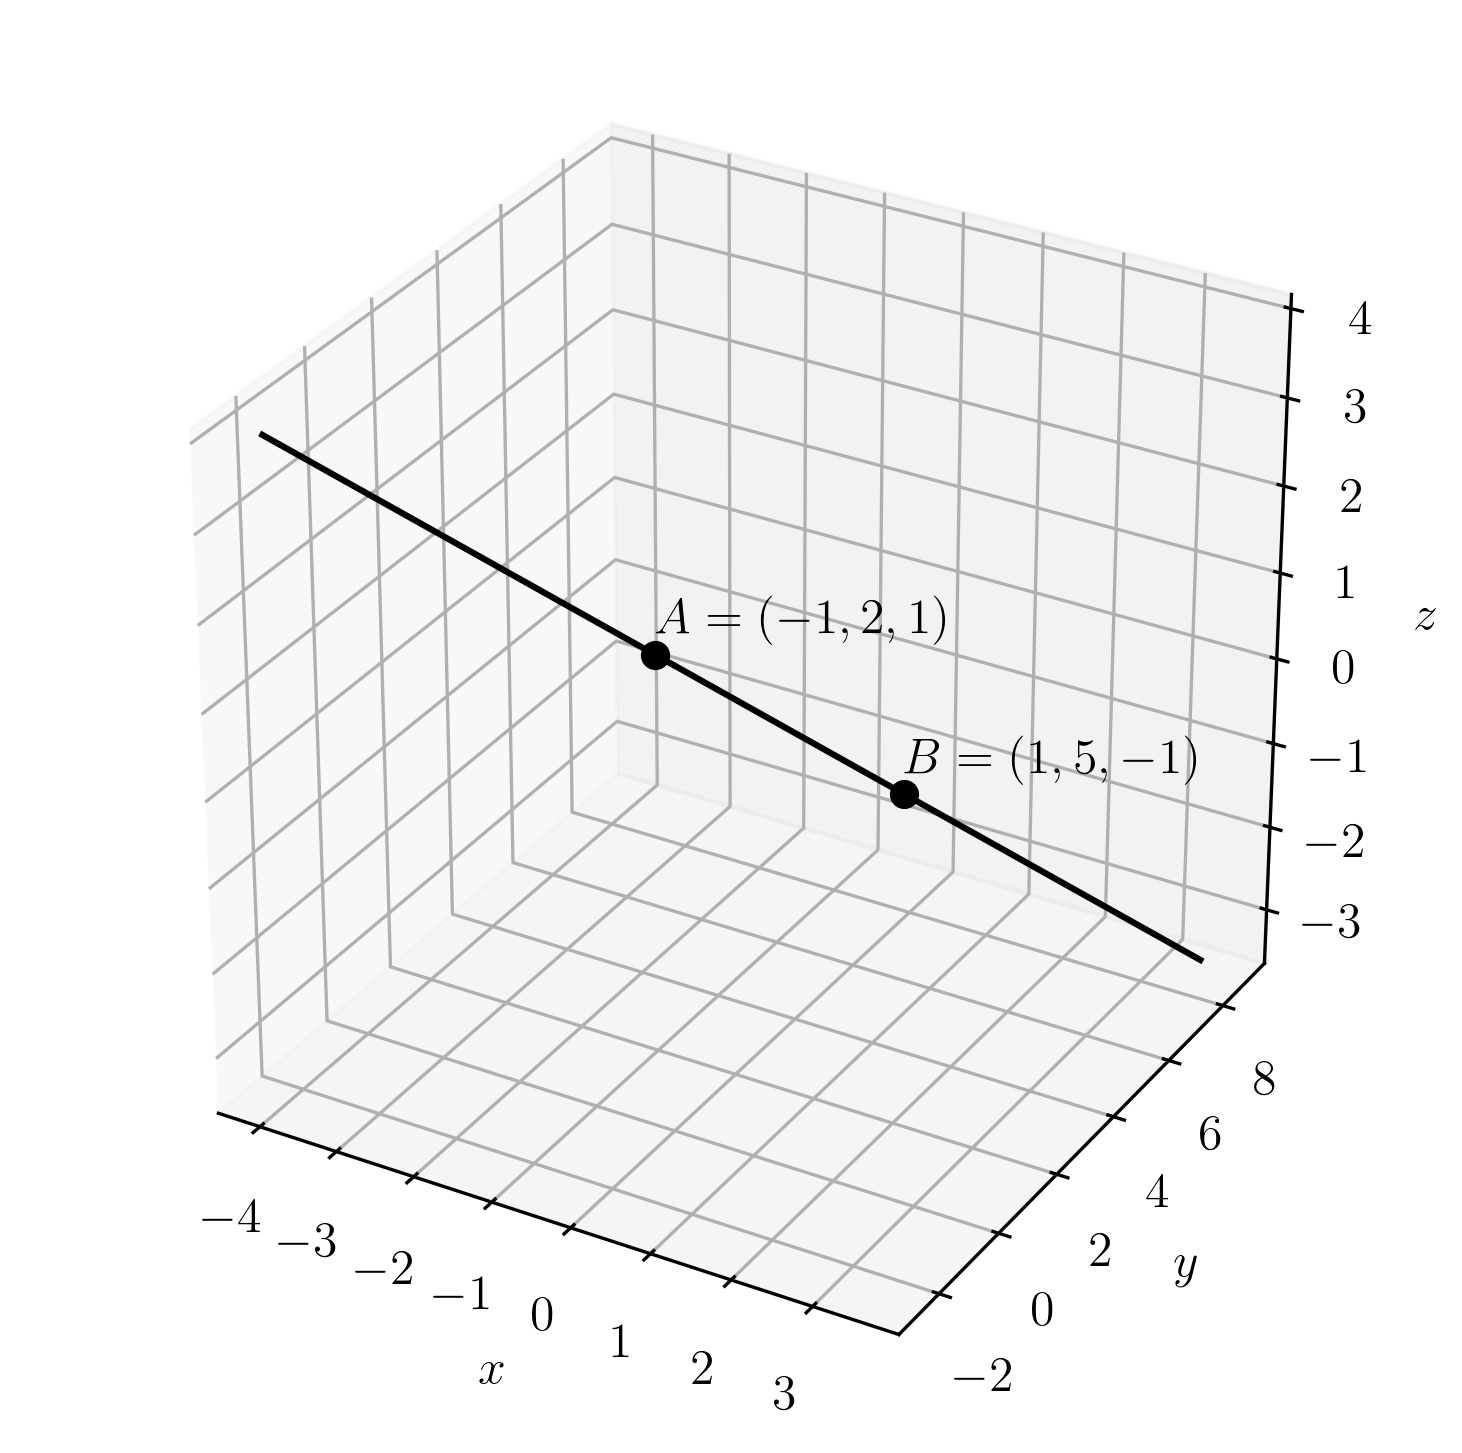
\includegraphics[width=0.7\textwidth]{./cap_er/dados/fig_exeresol_er_sim/fig_exeresol_er_sim}
    \caption{Esboço do gráfico da reta $r$ do Exercício Resolvido \ref{exeresol:er_sim}.}
    \label{fig:exeresol_er_sim}
  \end{figure}
\end{resol}